\documentclass[11pt]{article}
\usepackage[T1]{fontenc}
\usepackage{lmodern}
\usepackage{amsmath,amssymb,amsthm,mathtools}
\usepackage[margin=1.05in]{geometry}
\usepackage{microtype,fancyhdr,tikz,needspace}
\usetikzlibrary{arrows.meta}
\definecolor{linkblue}{RGB}{24,45,111}
\usepackage[colorlinks=true,allcolors=blue]{hyperref}
\newcommand{\C}{\mathbb C}
\newcommand{\R}{\mathbb R}
\newcommand{\D}{\mathbb D}
\newcommand{\T}{\mathbb T}
\newcommand{\cC}{\mathcal C}
\newcommand{\cH}{\mathcal H}
\newcommand{\M}{\mathsf M}
\newcommand{\HS}{\mathrm{HS}}
\DeclareMathOperator{\tr}{tr}
\DeclareMathOperator{\vecop}{vec}
\DeclareMathOperator{\dist}{dist}
\DeclareMathOperator{\diag}{diag}
\DeclareMathOperator{\spec}{spec}
\newtheorem{theorem}{Theorem}[section]
\newtheorem{corollary}[theorem]{Corollary}
\newtheorem{proposition}[theorem]{Proposition}
\newtheorem{lemma}[theorem]{Lemma}
\theoremstyle{definition}
\theoremstyle{remark}
\newtheorem{remark}[theorem]{Remark}
\numberwithin{equation}{section}
\pagestyle{fancy}\fancyhf{}
\fancyhead[L]{\small The complete Crouzeix theorem}
\fancyhead[R]{\small Structural route}
\fancyfoot[C]{\thepage}
\setlength{\headheight}{14pt}
\setlength{\emergencystretch}{2em}
\hypersetup{pdftitle={The complete Crouzeix theorem: optimal similarity and a common positive boundary representation},pdfauthor={OpenAI}}
\title{The complete Crouzeix theorem:\\
optimal similarity and a common positive boundary representation}
\author{OpenAI}
\date{September 23, 2026}
\begin{document}
\maketitle\thispagestyle{fancy}

\begin{abstract}
We resolve the complete Crouzeix conjecture by proving the sharp
constant-two numerical-range inequality for every bounded operator on a
complex Hilbert space and every matrix-valued polynomial. No separability
assumption is needed. The closure of the numerical range is a complete
$2$-spectral set, and the bound extends to finite matrix-valued functions
holomorphic near that closure. For a finite matrix and a bounded convex
domain containing its numerical range with regular real-analytic Jordan
boundary, the optimal similarity making its conformal disk image contractive
is attained with condition number at most two. For the similar matrix, one
continuous positive boundary density of mass the identity represents the
evaluation of every matrix-valued function holomorphic near the closed domain.
\end{abstract}

\section{The structural question}
Can one choose a single controlled change of inner product and a single
positive boundary density to represent all matrix-valued analytic evaluations
of a matrix? We answer this question on an analytic convex neighborhood of
its numerical range. The metric and density depend on the matrix and the
enclosing domain, but neither depends on the coefficient size or the function
being evaluated. The resulting complete inequality also holds for every
bounded operator on an arbitrary complex Hilbert space, by a finite
compression argument in Section~\ref{sec:limit}.

\subsection*{Coordinates and evaluation}
Write $\D=\{z\in\C:|z|<1\}$ and $\T=\partial\D$, with normalized
angular measure $d\sigma(e^{i\theta})=d\theta/(2\pi)$. For
$A\in M_n(\C)$ its numerical range is
\[
 W(A)=\{x^*Ax:x\in\C^n,\ x^*x=1\}.
\]
All operator norms are Hilbert-space operator norms, and tensor products are
Hilbert tensor products with the base space first. For a matrix-valued function $v$
holomorphic near the spectrum, $v[A]$ denotes holomorphic evaluation:
on a Jordan block $J=\beta I+N$ of size $s$ it is
$\sum_{j=0}^{s-1}N^j\otimes v^{(j)}(\beta)/j!$, followed by the
change of basis on the first factor. In particular,
$v[A]=\sum_jA^j\otimes B_j$ when $v(z)=\sum_jB_jz^j$.
Inner products are conjugate-linear in the first argument, and $U\preceq V$
means that $V-U$ is positive semidefinite. The symbol ${}^*$ denotes the
adjoint on a base or coefficient Hilbert space, ${}^{\mathsf T}$ ordinary
transpose, and ${}^\dagger$ the adjoint of an operator on a function space.

Call $\Omega$ \emph{admissible} when it is a bounded open convex subset of
$\C$ with regular real-analytic Jordan boundary.

\Needspace{9\baselineskip}
\begin{lemma}[Conformal coordinates]\label{lem:conformal-coordinates}
For every admissible $\Omega$ there is a conformal bijection
$f:\Omega\to\D$ such that $f$ and $f^{-1}$ extend univalently
through $\overline\Omega$ and $\overline\D$, respectively. There is also
a conformal bijection $G:\{|t|>1\}\to\C\setminus\overline\Omega$
that extends univalently to
$\{|t|>r\}\cup\{\infty\}$ for some $0<r<1$, as a sphere map, with a
simple pole at infinity and $G(\T)=\partial\Omega$. On $\T$, $tG'(t)$ is an outward normal and
$\psi=f\circ G$ is an orientation-preserving smooth circle diffeomorphism.
\end{lemma}
The complete local Riemann-mapping, harmonic-reflection, and collar argument
is in Appendix~\ref{sec:conformal-appendix}.


Fix such an $\Omega$ with $W(A)\subset\Omega$, and choose its coordinates
$f,G$ from Lemma~\ref{lem:conformal-coordinates}. Put $T=f(A)$ and define
\begin{equation}\label{eq:minimum}
 \kappa^2=\min\{\tau\in\R:I\preceq H\preceq\tau I,
                  \ T^*HT\preceq H\text{ for some }H=H^*\}.
\end{equation}
A strictly feasible pair means that $H-I$, $\tau I-H$, and
$H-T^*HT$ are all positive definite. Existence and attainment of the
minimum are part of the first conclusion.

\begin{theorem}[The optimal metric]\label{thm:structural}
For every admissible $\Omega$, every finite $n\ge1$, every
$A\in M_n(\C)$ with $W(A)\subset\Omega$, and the interior conformal
coordinate $f$ above, the problem \eqref{eq:minimum} is strictly feasible
and has an attained minimum $1\le\kappa^2\le4$. If $H$ is a minimizing
metric, then
\[
 S=H^{1/2},\qquad A'=SAS^{-1},\qquad D=Sf(A)S^{-1}=f(A')
\]
satisfy
\[
 D^*D\preceq I,\qquad \rho(D)<1,
 \qquad \|S\|\|S^{-1}\|=\kappa\le2.
\]
\end{theorem}

\begin{theorem}[A common positive representation]\label{thm:representation}
With the same $\Omega,A,f,G$ and any chosen minimizing metric in
Theorem~\ref{thm:structural}, there is one continuous function
$\Lambda:\T\to M_n(\C)$ satisfying
\[
 \Lambda(t)\succeq0,\qquad \int_\T\Lambda(t)\,d\sigma(t)=I_n,
\]
such that, for every positive integer $m$ and every $M_m(\C)$-valued
function $v$ holomorphic on a neighborhood of $\overline\Omega$,
\begin{equation}\label{eq:representation-target}
 v[A']=\int_\T\Lambda(t)\otimes v(G(t))\,d\sigma(t),
 \qquad
 \|v[A]\|\le\kappa\max_{\overline\Omega}\|v\|.
\end{equation}
The same $S$, $\Lambda$, and $\kappa$ work for all $m$ and $v$.
\end{theorem}

\subsection*{The complete inequality and previous work}
For a bounded operator $A$ on a nonzero complex Hilbert space $\mathcal H$,
write $W(A)=\{\langle x,Ax\rangle:\|x\|=1\}$. For a matrix polynomial
$P(z)=\sum_{j=0}^dB_jz^j$, with $B_j\in M_m(\C)$, put
$P[A]=\sum_{j=0}^dA^j\otimes B_j$ on $\mathcal H\otimes\C^m$.
The operator formulation of the complete Crouzeix conjecture asks whether
$\|P[A]\|\le2\sup_{W(A)}\|P\|$ holds independently of the Hilbert
space, the finite coefficient size $m$, and the degree $d$. The scalar
problem is the case $m=1$.
Theorems~\ref{thm:structural} and~\ref{thm:representation}, together with
analytic convex outer approximation, give the finite-matrix inequality in
Corollary~\ref{cor:polynomial}. Corollary~\ref{cor:hilbert} transfers it
to all bounded Hilbert-space operators, including those on nonseparable
spaces, and gives the corresponding rational and holomorphic bounds on
$\overline{W(A)}$. The optimal similarity and the common density are the
finite-dimensional structural conclusions proved before these passages.

Crouzeix formulated the scalar constant-two question in 2004 and obtained
a universal complete bound of $11.08$ in 2007
\cite{Crouzeix2004,Crouzeix2007}. Delyon and Delyon's positive integral
representations form an important part of the numerical-range method
\cite{DelyonDelyon1999}. Crouzeix and Palencia used a positive double-layer
potential and a conjugate-data Cauchy transform to obtain the complete
bound $1+\sqrt2$ \cite{CrouzeixPalencia2017}; Ransford and Schwenninger
simplified its final norm argument \cite{RansfordSchwenninger2018}.
Recent preprints by Jin, Lorist and Schwenninger, and Luo present
scalar constant-two proofs \cite{Jin2026,LoristSchwenninger2026,Luo2026}.
Lorist and Schwenninger's Theorem~3 covers bounded Hilbert-space operators;
their Section~3(iv) explains why its commutation argument does not
immediately pass to matrix coefficients. \AA hag, Czy{\.{z}}, and Virtanen
prove the complete constant-two estimate for base matrices of order at
most three, with arbitrary coefficient size
\cite[Theorem~1.1]{AhagCzyzVirtanen2026}. The present comparison retains
both matrix multiplication orders in all finite base dimensions, which
suffices for the bounded-operator consequence by compression.

The abstract connection with controlled similarity is classical. Paulsen's
similarity theorem identifies the optimal condition number with the completely
bounded norm \cite[Section 2, unnumbered theorem]{Paulsen1984Similarity};
Arveson's dilation theorem relates complete contractivity to a normal boundary
dilation \cite[Theorem 1.2.2]{Arveson1972}. For numerical-range ellipses in
base dimension two, Badea, Crouzeix, and Delyon construct a conformal similarity
with condition number at most two
\cite[Theorem 5.2 and Corollary 5.3]{BadeaCrouzeixDelyon2006}.
Here we construct the minimizing metric, its endpoint extremal data, and the
continuous density in a fixed boundary parameter, and prove $\kappa\le2$
for the optimal metric constant in \eqref{eq:minimum}.

The direct proof in \cite{Direct} reaches the polynomial inequality
from the singular vectors of the polynomial being evaluated. Its exterior
kernel and original-matrix resolvent calculations also occur here, with
complete local proofs. The present argument instead chooses one optimal
metric first and proves a representation valid for every coefficient size
and every analytic test function. The two manuscripts have separate
complete proof paths.

\subsection*{How the two conclusions are proved}
Section~\ref{sec:metric} first attains the metric minimum and constructs
its positive disk density before estimating $\kappa$. The boundary change
of coordinates
\[
 t\in\T\ \xrightarrow{\ G\ }\ G(t)\in\partial\Omega
 \ \xrightarrow{\ f\ }\ \psi(t)\in\T
\]
has a positive angular Jacobian. Including it in the density gives
$\Lambda$. Its mass-one identity makes the map
$b\mapsto[t\mapsto(\Lambda(t)^{1/2}\otimes I_m)b]$ an isometric
embedding of $\C^n\otimes\C^m$ into boundary $L^2$ functions.
Multiplying there by $I_n\otimes v(G(t))$ and applying the embedding's
adjoint gives $v[A']$. This is the common compression at every coefficient size.
Figure~\ref{fig:coordinates} displays the two boundary parameters.

\begin{figure}[htbp]
\centering
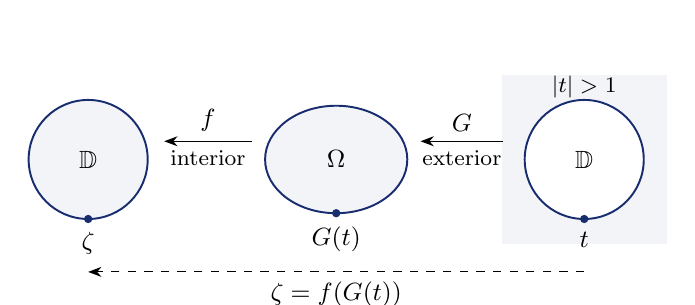
\begin{tikzpicture}[x=1.05cm,y=1.05cm,>=Stealth,
  every node/.style={font=\small},
  coordinate curve/.style={draw=linkblue,line width=.7pt}]
  \fill[linkblue!5] (-3,0) circle (.72);
  \draw[coordinate curve] (-3,0) circle (.72);
  \node at (-3,0) {$\D$};
  \fill[linkblue!5] (0,0) ellipse (.86 and .65);
  \draw[coordinate curve] (0,0) ellipse (.86 and .65);
  \node at (0,0) {$\Omega$};
  \fill[linkblue!5] (2,-1.02) rectangle (4,1.02);
  \fill[white] (3,0) circle (.72);
  \draw[coordinate curve] (3,0) circle (.72);
  \node at (3,0) {$\D$};
  \node[font=\footnotesize] at (3,.88) {$|t|>1$};
  \draw[->] (-1.02,.22) -- node[above] {$f$}
    node[below,font=\footnotesize] {interior} (-2.08,.22);
  \draw[->] (2.02,.22) -- node[above] {$G$}
    node[below,font=\footnotesize] {exterior} (1.02,.22);
  \fill[linkblue] (-3,-.72) circle (1.5pt);
  \fill[linkblue] (0,-.65) circle (1.5pt);
  \fill[linkblue] (3,-.72) circle (1.5pt);
  \node[below] at (-3,-.76) {$\zeta$};
  \node[below] at (0,-.70) {$G(t)$};
  \node[below] at (3,-.76) {$t$};
  \draw[->,dashed] (3,-1.36) -- node[below] {$\zeta=f(G(t))$} (-3,-1.36);
\end{tikzpicture}
\caption{The two conformal coordinates, shown schematically; $\Omega$ need not
be an ellipse. The Cauchy projection uses the
exterior boundary parameter $t$ and its uniform circle measure. The
contraction representation uses the interior disk coordinate $\zeta$;
passing between them requires the positive Jacobian of the boundary map
$f\circ G$. The shaded exterior on the right is the domain of $G$.}
\label{fig:coordinates}
\end{figure}



If $\kappa>1$, finite-dimensional separation supplies unit vectors
$x,y\in\C^n\otimes\C^n$ in the $\kappa$ and $1$ eigenspaces of
$S\otimes I_n$, respectively. A unitary realization gives a contractive
$M_n(\C)$-valued disk function $F_\D$ with $F_\D[D]x=y$.
This auxiliary function has coefficient
size $n$; its role is to test one base-space metric, not to restrict the
independently chosen target size $m$.

Once the extremal vectors are available, Section~\ref{sec:inputs}
introduces the local boundary tools needed to compare them: the exterior
kernel, the actual Cauchy adjoint, both analytic multiplication orders,
and the positive resolvent of the original $A$. In
Section~\ref{sec:bridge}, equality in the common compression gives the
forward and adjoint relations between the
boundary vectors $x_\Lambda(t)=(\Lambda(t)^{1/2}\otimes I_n)x$ and
$y_\Lambda(t)=(\Lambda(t)^{1/2}\otimes I_n)y$.
Partial traces of their outer products sum the diagonal base-space blocks,
leaving coefficient-space matrix fields. An ordinary transpose fixed by
the tensor convention identifies their means, including an entirely
vanishing matrix cross mean. The original-$A$ resolvent produces
a second positive block. Analytic and adjointed cross tests relate the
two blocks with factors $\kappa$ and $\kappa^{-1}$, respectively.

The decisive comparison is between the cross density and the two diagonal
densities in this second positive block. We use boundary $L^2$ norms formed
with the Hilbert--Schmidt matrix norm. Positivity bounds twice the squared
norm of the cross density by the sum of the squared norms
of the diagonal densities. Both diagonal norms are controlled by the same
nonzero projected cross density from the first system. The zero matrix mean
separates the two projected cross terms into orthogonal Fourier subspaces,
so the factor $\kappa$ gives a lower bound for the second cross density.
Section~\ref{sec:comparison} combines these bounds to prove $\kappa\le2$.
This completes the metric theorem and returns to
the common density at every target size. Section~\ref{sec:limit} applies
the result to polynomials and passes to arbitrary finite-matrix numerical
ranges, including points and segments. It then uses finite compressions
and holomorphic approximation to obtain the complete inequality for bounded
operators on arbitrary complex Hilbert spaces.
Appendix~\ref{sec:conformal-appendix}
provides the full local conformal construction used throughout.

\section{The metric, its representation, and its extremal data}\label{sec:metric}
\subsection{A metric for the disk coordinate}
The evaluation rules used below follow directly from the finite Jordan
Taylor formula. Its product rule preserves the order of matrix coefficients;
conjugating the Jordan form proves similarity on the base factor. For scalar
composition, substitute the nilpotent matrix $f(J)-f(\beta)I$ into the
Taylor series of the outer function at $f(\beta)$. The finite Taylor
composition identity gives $(v\circ f)[J]=v[f(J)]$, and the same formula
gives $\spec(f(A))=f(\spec(A))$. No diagonalizability is assumed.
The Jordan resolvent expansion and Cauchy's derivative formula give the
equivalent contour-integral evaluation.

Since $\spec(A)\subset W(A)\subset\Omega$, spectral mapping gives
$\rho(T)<1$. The positive-metric feasibility criterion is classical
\cite[Theorem 1]{Stein1952}; we construct the strictly feasible witness.
Choose $\rho(T)<\eta<1$. Jordan normal form supplies
$C_\eta$ with $\|T^j\|\le C_\eta\eta^j$. Hence
\[
 H_0=\sum_{j\ge0}T^{*j}T^j
\]
converges in norm, $H_0\succeq I$, and $H_0-T^*H_0T=I$.
For $c>1$ and $\tau>\|cH_0\|$, the pair $(\tau,cH_0)$ has all
three matrix slacks in \eqref{eq:minimum} positive definite. This is
strict feasibility of the optimization problem. Feasible pairs below any
fixed feasible upper bound form a closed bounded subset of a finite-dimensional
space, so a minimum is attained. Every feasible $\tau$ is at least one.

Fix a minimizing $H$ and put $S=H^{1/2}$. Congruence gives
$D^*D=S^{-1}T^*HTS^{-1}\preceq I$; similarity gives $\rho(D)<1$.
The inequalities $I\preceq H\preceq\kappa^2I$ give
$\|S\|\|S^{-1}\|\le\kappa$. The optimizer itself may have zero
slacks. In particular $\|D\|=1$ is allowed.

The minimum also measures the best condition number of a similarity to
a contraction. If $R$ is invertible and $\|RTR^{-1}\|\le1$, then
$H_R=R^*R$ satisfies $T^*H_RT\preceq H_R$. Dividing $H_R$ by its
least eigenvalue gives a feasible metric with
$\tau=\|R\|^2\|R^{-1}\|^2$. Consequently
$\kappa\le\|R\|\|R^{-1}\|$. Applying this to the minimizing
$S=H^{1/2}$, for which the reverse inequality was just proved, gives
\begin{equation}\label{eq:optimal-similarity}
 \kappa=\min\{\|R\|\|R^{-1}\|:
 R\text{ invertible},\ \|RTR^{-1}\|\le1\}.
\end{equation}
The minimum is attained by the positive matrix $S$, with
$\|S\|\|S^{-1}\|=\kappa$. This identity holds for any fixed finite
$T$ with an attained feasible metric problem; the stability assumption
above supplies such feasibility. The bound $\kappa\le2$ proved below
uses the additional conformal and numerical-range hypotheses.

\subsection{One density for every coefficient size}
\begin{proposition}[One density for every coefficient size]\label{prop:density}
For the fixed minimizing metric, the representation
\eqref{eq:representation-target} holds, before any bound on $\kappa$ is
proved, with
\begin{align}
 \Phi_D(\zeta)&=(I-D/\zeta)^{-1}+[(I-D/\zeta)^{-1}]^*-I,
                                                        \label{eq:phi}\\
 j(t)&=\frac{tG'(t)f'(G(t))}{\psi(t)}>0,
 &\Lambda(t)&=j(t)\Phi_D(\psi(t)).                      \label{eq:lambda}
\end{align}
\end{proposition}
The disk-resolvent formula is the positive representation of
Delyon and Delyon \cite[Section 2, equation (7)]{DelyonDelyon1999};
the common compression also belongs to the dilation tradition
\cite[Theorem I]{SzNagy1953}. We express the density in the exterior
parameter and prove every coefficient-size claim.
\begin{proof}
For $|\zeta|=1$, $E_\zeta=I-D/\zeta$ is invertible and
\[
 E_\zeta^*\Phi_D(\zeta)E_\zeta=I-D^*D\succeq0.
\]
Thus $\Phi_D$ is positive and continuous. The strict spectral-radius
bound, rather than a strict norm bound, implies $\sum_{j\ge0}\|D^j\|<\infty$.
Consequently the following series is absolutely uniformly convergent on
the circle:
\[
 \Phi_D(\zeta)=I+\sum_{j\ge1}(\zeta^{-j}D^j+\zeta^jD^{*j}),
 \qquad \int_\T\zeta^j\Phi_D(\zeta)\,d\sigma(\zeta)=D^j
 \quad(j\ge0).
\]
For any $m$ and any $M_m$-valued $h$ holomorphic near $\overline\D$,
integration of its uniformly convergent Taylor series gives
\[
 h[D]=\int_\T\Phi_D(\zeta)\otimes h(\zeta)\,d\sigma(\zeta).
\]
Apply this with $h=v\circ f^{-1}$. The conformal collar makes $h$
holomorphic near $\overline\D$, and scalar composition gives $h[D]=v[A']$.
Locally writing $\psi(e^{i\theta})=e^{i\eta(\theta)}$ shows that
$j(e^{i\theta})=\eta'(\theta)>0$. Changing variables
$\zeta=\psi(t)$ proves the first identity in
\eqref{eq:representation-target}. The zeroth moment gives
$\int\Lambda\,d\sigma=I$.

For each $m$, define
\[
 V_m:\C^n\otimes\C^m\longrightarrow
 L^2(\T,d\sigma;\C^n\otimes\C^m),\qquad
 (V_m b)(t)=(\Lambda(t)^{1/2}\otimes I_m)b.
\]
Normalization makes $V_m$ an isometry. If $M_v$ multiplies by
$I_n\otimes v(G(t))$, then
\[
 v[A']=V_m^\dagger M_vV_m,\qquad
 \|v[A']\|\le\max_{\overline\Omega}\|v\|.
\]
Similarity on the first factor gives the remaining estimate with constant
$\kappa$. Neither the definition of $S$ nor that of $\Lambda$ depends
on $m$ or $v$.
\end{proof}

\subsection{Endpoint separation and an exact extremal}
To bound the metric, we need equality for one auxiliary matrix function.
The construction passes from real separation to a dual balance, then to
endpoint supports, and finally to a finite unitary realization.
Use the vectorization convention
\[
 \vecop(X)=\sum_{j=1}^nXe_j\otimes e_j,\qquad
 \|\vecop(X)\|^2=\tr(XX^*).
\]

\begin{proposition}[Endpoint extremal]\label{prop:extremal}
If $\kappa>1$, there are $X,Y\in M_n(\C)$ with
\[
 \tr(XX^*)=\tr(YY^*)=1,\qquad SX=\kappa X,\qquad SY=Y,
 \qquad X^*Y=0,
\]
and an $M_n$-valued rational function $F_\D$, holomorphic on a neighborhood
of $\overline\D$ and contractive on $\overline\D$, such that, for
$x=\vecop(X)$ and $y=\vecop(Y)$,
\[
 F_\D[D]x=y.
\]
In particular $F_\Omega=F_\D\circ f$ is holomorphic near
$\overline\Omega$ and satisfies $F_\Omega[A']x=y$. Its boundary trace
$F=F_\Omega\circ G$ is contractive.
\end{proposition}
\begin{proof}
We first obtain positive matrices $X_0$ and $Y_0$ supported on the
$\kappa^2$ and $1$ eigenspaces of $H$, respectively. A third positive
matrix $Z_0$ will express their difference as $Z_0-TZ_0T^*$; this balance
will provide the equal Gram matrices needed for the unitary realization.

\emph{Separation, including a possible contact point.}
In the real vector space $\R\oplus\operatorname{Herm}_n^3$, the affine set
\[
 \mathcal A_T=\{(s,J-I,sI-J,J-T^*JT):s\in\R,\ J=J^*\}
\]
is disjoint from the open convex set
\[
 \mathcal O=\{(s,U,V,W):s<\kappa^2,\ U,V,W\succ0\}.
\]
Here is the finite-dimensional separation argument used for these sets;
the general convex-separation framework is treated in
\cite[Section 11, Theorem 11.2]{Rockafellar1970}.
Write $\mathcal A_T=a_0+L$, and let $\pi$ project orthogonally onto
$L^\perp$. The set $\mathcal K=\pi(\mathcal O-a_0)$ is nonempty, open
in $L^\perp$, and convex, and it does not contain zero. If
$0\notin\overline{\mathcal K}$, a nearest point $z_0$ in the closed convex
set $\overline{\mathcal K}$ satisfies
$\langle z_0,c\rangle\ge\|z_0\|^2>0$ for every $c\in\mathcal K$.

If $0\in\overline{\mathcal K}$, fix $c_*\in\mathcal K$ and set
$z_j=-c_*/j$. Each $z_j$ is outside $\overline{\mathcal K}$: otherwise
zero would lie on the open segment joining an interior point $c_*$ to a
point of the closure, and hence would belong to $\mathcal K$. To verify
that segment fact, take a ball about $c_*$ inside $\mathcal K$, approximate
the other endpoint by points of $\mathcal K$, and use convexity; a ball
about each fixed interior point of the limiting segment is still contained
in $\mathcal K$. Let $y_j$ be nearest to $z_j$ in
$\overline{\mathcal K}$. Since zero belongs to this closed set,
$\|y_j-z_j\|\le\|z_j\|$, so $y_j\to0$. A subsequence of
$\nu_j=(y_j-z_j)/\|y_j-z_j\|$ tends to a unit vector $\nu$.
The nearest-point inequality gives
$\langle\nu_j,c-y_j\rangle\ge0$, hence
$\langle\nu,c\rangle\ge0$ for every $c\in\mathcal K$.
In the first case use $\nu=z_0$. In either case
$\ell(v)=-\langle\nu,\pi v\rangle$ is nonzero and
$\ell(a)\ge\ell(o)$ for all $a\in\mathcal A_T$, $o\in\mathcal O$.

Because $\mathcal A_T$ is affine, $\ell$ is constant on it. Boundedness
above on $\mathcal O$ forces the signs
\[
 \ell(s,U,V,W)=\lambda s-\tr(Y_0U)-\tr(X_0V)-\tr(Z_0W),
 \quad\lambda\ge0,\quad X_0,Y_0,Z_0\succeq0.
\]
If $\lambda=0$, strict feasibility produces a negative value on
$\mathcal A_T$, while separation requires a value at least
$\sup_{\mathcal O}\ell=0$. Thus $\lambda>0$; scale it to one.
Constancy on $\mathcal A_T$ then gives
\begin{equation}\label{eq:dual}
 X_0-Y_0=Z_0-TZ_0T^*,\qquad \tr X_0=1.
\end{equation}
The constant value is $\tr Y_0\ge\kappa^2$. At $(\kappa^2,H)$ it is
\[
 \kappa^2-\tr(Y_0(H-I))-\tr(X_0(\kappa^2I-H))
            -\tr(Z_0(H-T^*HT))\le\kappa^2.
\]
Each subtracted trace is nonnegative, so all vanish and
$\tr Y_0=\kappa^2$.

\emph{Endpoint support and balance.}
Write
$\|B\|_{\HS}=(\tr(B^*B))^{1/2}$ for the unnormalized
Hilbert--Schmidt norm. For positive matrices $B,C$,
$\tr(BC)=\|C^{1/2}B^{1/2}\|_{\HS}^2$; vanishing implies that the
range of $B$ lies in the kernel of $C$. Therefore $X_0$ is supported on
the $\kappa^2$ eigenspace of $H$, and $Y_0$ on its $1$ eigenspace.

Choose square factors and a positive matrix $Q$ by
\[
 XX^*=\kappa^{-2}SX_0S,\quad
 YY^*=\kappa^{-2}SY_0S,\quad Q=\kappa^{-2}SZ_0S.
\]
The support and trace relations give the asserted norms and endpoint
identities. Their column ranges are orthogonal because $\kappa>1$,
so $X^*Y=0$ as a matrix. Congruence of \eqref{eq:dual} gives
\begin{equation}\label{eq:balance}
 XX^*-YY^*=Q-DQD^*.
\end{equation}

\emph{Unitary realization and transpose.}
The balance-to-isometry step is the classical interpolation mechanism of
\cite[Section~3 of the versioned preprint]{KatsnelsonKheifetsYuditskii1997}; its particular endpoint
data and finite-dimensional realization are established here.
Put $L=Q^{1/2}$. The rows $R_1=[L\ Y]$ and $R_2=[DL\ X]$ have
equal products with their adjoints. The map
$R_2^*v\mapsto R_1^*v$ is therefore a well-defined isometry of their
ranges. Extend it to a unitary using equal-dimensional orthogonal
complements, then take its adjoint. This yields
\[
 [L\ Y]=[DL\ X]
 \begin{pmatrix}a&b\\c&d\end{pmatrix},\qquad
 U=\begin{pmatrix}a&b\\c&d\end{pmatrix}\text{ unitary}.
\]
Thus $L=DLa+Xc$ and $Y=DLb+Xd$. Since $\|a\|\le1$ and
$\rho(D)<1$, iteration gives the norm-convergent identity
\begin{equation}\label{eq:realization-series}
 Y=Xd+\sum_{j\ge0}D^{j+1}Xca^jb.
\end{equation}
The transfer-function norm identity is the unitary-colligation identity
of \cite[Section 3.1, equations (3.1)--(3.4)]{Brodskii1978}.
Define, for $|\zeta|<1$,
\[
 R(\zeta)=d+\zeta c(I-\zeta a)^{-1}b,
 \qquad F_\D(\zeta)=R(\zeta)^{\mathsf T}.
\]
For $e\in\C^n$ and $v=(I-\zeta a)^{-1}be$, unitarity gives
\[
 U\binom{\zeta v}{e}=\binom{v}{R(\zeta)e},\qquad
 \|e\|^2-\|R(\zeta)e\|^2=(1-|\zeta|^2)\|v\|^2\ge0.
\]
Hence $R$ is contractive. Ordinary transpose preserves its norm and
holomorphy. Its rational entries are bounded in $\D$, so every apparent
pole on $\T$ is removable: a genuine pole would diverge on an interior
radial approach. After cancellation, finitely many remaining poles stay
away from $\overline\D$. This supplies a common neighborhood of that
closed disk on which $F_\D$ is holomorphic; continuity retains
contractivity on the circle.

Finally,
\[
 (D^k\otimes B)\vecop(X)=\vecop(D^kXB^{\mathsf T}).
\]
The Taylor coefficients of $F_\D$ are the transposes of $d$ and
$ca^jb$. Substitution in \eqref{eq:realization-series} proves
$F_\D[D]x=y$. The conformal collar and scalar composition give the
claims for $F_\Omega$. Rationality is asserted in the disk variable;
$F_\Omega$ is only required to be holomorphic near $\overline\Omega$.
\end{proof}

\section{Local boundary tools}\label{sec:inputs}
We now prepare the comparison that will bound the optimal metric. The
exterior coordinate supplies a positive kernel with two normalized marginals.
Its Fourier action controls a Cauchy projection, while the original numerical
range supplies a second positive density. We prove the shared exterior and
resolvent calculations here. They also form the analytic part of the direct
polynomial proof \cite[Sections 2--3]{Direct}; each required argument is
included in the present paper. A reader who has checked
\cite[Theorems~2.1 and~3.1]{Direct} may compare the statement of
Proposition~\ref{input:analytic} using the notation in
Remark~\ref{rem:correspondence}, and then resume at the physical Cauchy
integral preceding Proposition~\ref{prop:projection}. The projection
proof and its ordered applications remain part of the present argument.

\begin{proposition}[Exterior coefficients and the original-matrix resolvent]\label{input:analytic}
Assume the admissible $\Omega$ and the exterior map $G$ supplied above.
Write $G(t)=at+b+O(t^{-1})$ at infinity, where $a\ne0$, and
$q_G(t)=tG'(t)$. There are scalar polynomials
$b_k$, with $b_0=1$, $\deg b_k=k$, and leading coefficient $a^{-k}$,
defined by
\begin{equation}\label{eq:import-faber}
 \frac{q_G(t)}{G(t)-z}=\sum_{k\ge0}b_k(z)t^{-k}
 \quad\text{at infinity}.
\end{equation}
There is also the mixed expansion
\begin{equation}\label{eq:import-kernel}
 B(w,t)=\frac{q_G(t)}{G(t)-G(w)}-\frac{t}{t-w}
       =\sum_{i,j\ge1}\beta_{ij}w^{-i}t^{-j},
 \qquad
 b_j(G(w))=w^j+\sum_{i\ge1}\beta_{ij}w^{-i}\quad(j\ge1).
\end{equation}
Here $B$ is holomorphic through the diagonal and both infinities of the
exterior product collar. For each $r<\rho<1$ there is a constant
$C_\rho$ such that $|\beta_{ij}|\le C_\rho\rho^{i+j}$; the series
converges normally on the product collar and absolutely uniformly on
$\T^2$. The kernel
\[
 m(w,t)=1+B(w,t)+\overline{B(w,t)}
\]
is continuous and nonnegative, with each normalized-circle marginal one.

For every finite $n$ and every original matrix $A\in M_n(\C)$ with
$W(A)\subset\Omega$,
\begin{equation}\label{eq:import-resolvent}
 K_A(t)=q_G(t)(G(t)I-A)^{-1}
       =\sum_{k\ge0}b_k(A)t^{-k},\qquad
 E_A(t)=K_A(t)+K_A(t)^*\succeq0\quad(t\in\T).
\end{equation}
Its coefficients decay geometrically and its series converges absolutely
uniformly on $\T$.
The scalar case applies to every fixed $z\in\Omega$.
\end{proposition}
\begin{proof}
Expand \eqref{eq:import-faber} at infinity after factoring $at$ from the
denominator. The constant term is one; the coefficient of $t^{-k}$ is a
polynomial of degree $k$ with leading term $a^{-k}z^k$.

For the joint continuation, put
\[
 Q(w,t)=\frac{G(t)-G(w)}{t-w}.
\]
Write $u=t^{-1}$, $v=w^{-1}$, and $G(t)=at+g(u)$, with $g$
holomorphic for $|u|<r^{-1}$. Then
\[
 Q=a-uv\frac{g(u)-g(v)}{u-v}.
\]
The divided difference is jointly holomorphic, with its derivative value
on the diagonal. Off the finite diagonal, $Q\ne0$ by univalence of
$G$; on that diagonal $Q=G'(t)\ne0$; on either reciprocal axis,
including their intersection, $Q=a\ne0$. Consequently
\[
 B(w,t)=t\frac{\partial_tQ(w,t)}{Q(w,t)}
        =-u\frac{\partial_uQ}{Q}
\]
is holomorphic on the reciprocal bidisk and vanishes on both axes.
Its Taylor series has only the strictly mixed powers in
\eqref{eq:import-kernel}. Cauchy estimates on the closed reciprocal
bidisk of radius $\rho^{-1}$ give
$|\beta_{ij}|\le C_\rho\rho^{i+j}$ for every $r<\rho<1$.
For a compact subset of the product collar, choose $\rho$ above $r$
but smaller than one and than the moduli of both coordinates on that
compact set. The estimate then dominates the double series by a product
of convergent geometric series. This proves normal convergence throughout
the product collar, including at infinity, and absolute uniform convergence
on $\T^2$.
Comparing coefficients at $t=\infty$ in the defining identity for $B$,
first with fixed finite $w$ in the collar, gives the displayed boundary
formula for $b_j\circ G$.

For distinct $w,t\in\T$, the circle identity
$2\operatorname{Re}(t/(t-w))=1$ gives
\[
 m(w,t)=2\operatorname{Re}\frac{q_G(t)}{G(t)-G(w)}\ge0.
\]
Indeed $q_G(t)$ is the outward normal, so convexity gives
$\operatorname{Re}(\overline{q_G(t)}(G(t)-G(w)))\ge0$.
Continuity of the mixed-series expression supplies the same sign on the
diagonal. Every term in $B$ and its conjugate has nonzero frequency in
each variable, so integration in either variable leaves exactly one.

For the matrix resolvent, every eigenvalue of $A$ lies in $W(A)$ by
testing a unit eigenvector. Thus $G(t)I-A$ is invertible on and outside
the circle. Compactness of the circle permits a smaller exterior collar
on which the resolvent remains holomorphic, including infinity where
$K_A(\infty)=I$. Expanding for large $|t|$ gives the coefficients
$b_k(A)$ by the same polynomial identities as \eqref{eq:import-faber}.
Cauchy estimates in the reciprocal disk give geometric decay and
absolute uniform convergence on $\T$.

Finally put $R_t=G(t)I-A$. Direct congruence gives
\[
 R_t^*(K_A+K_A^*)R_t=q_G(t)R_t^*+\overline{q_G(t)}R_t.
\]
At a unit vector $x$, its quadratic form is
$2\operatorname{Re}(\overline{q_G(t)}(G(t)-x^*Ax))\ge0$,
by the supporting half-plane and $W(A)\subset\Omega$.
Invertibility of $R_t$ proves $E_A\succeq0$.
\end{proof}

These local double-layer calculations belong to the numerical-range
method of Delyon--Delyon and Crouzeix--Palencia
\cite{DelyonDelyon1999,CrouzeixPalencia2017}.
The polynomials $b_k$ are the classical Faber polynomials
\cite{Beckermann2005,BeckermannCrouzeix2014}. Indeed, putting
$\Phi=G^{-1}$ in the exterior, \eqref{eq:import-kernel} gives
$b_k(z)-\Phi(z)^k=O(z^{-1})$ at infinity; hence $b_k$ is the
polynomial part of $\Phi^k$. The mixed coefficients $\beta_{ij}$ are
differentiated Grunsky coefficients, as the logarithmic derivative of $Q$
in the proof shows. The classical coefficient normalization gives a
weighted inequality \cite[equations (1.1)--(1.3)]{BeckermannStylianopoulos2018};
the unweighted Hilbert--Schmidt contraction used here follows locally
from convexity and the two angular marginals.

We next turn this kernel into a bounded Cauchy projection on boundary
functions. For the density comparison we need estimates for its actual
adjoint and a formula relating Laurent tests to the original-matrix field
$E_A$.

For every integer $k\ge1$, use
\[
 \cH_k=L^2(\T,d\sigma;M_k(\C)),\qquad
 \langle u,v\rangle=\int_\T\tr(u^*v)\,d\sigma,
 \qquad\|u\|_2^2=\langle u,u\rangle.
\]
The pointwise norm is the unnormalized Hilbert--Schmidt norm. Let
$P_0,P_+,P_-$ be the orthogonal Fourier projections onto the constant,
strictly positive, and strictly negative frequencies, respectively, and write
$u=u_0+u_++u_-$ with $u_0=P_0u$, $u_+=P_+u$, $u_-=P_-u$.
Define
\[
 (\M u)(w)=\int_\T m(w,t)u(t)\,d\sigma(t).
\]

\begin{remark}[Correspondence with the direct proof]\label{rem:correspondence}
A reader who has already checked the exterior calculations in
\cite[Theorems~2.1 and~3.1]{Direct} can compare the conventions by setting
$h=G$, $\lambda=t$, $\mu=w$. Its correction satisfies
$s(\lambda,\mu)=B(\mu,\lambda)$ and $s_{kj}=\beta_{jk}$.
The resulting integral action is the same $\M$, not its
Hilbert adjoint. The local proof above is complete; readers familiar with
that calculation can continue with the physical Cauchy interpretation below.
\end{remark}

For continuous matrix-valued boundary data $u$, define the physical
Cauchy integral
\[
 c_u(z)=\int_\T u(t)\frac{q_G(t)}{G(t)-z}\,d\sigma(t),\qquad z\in\Omega.
\]
For finite Laurent data, the scalar case of \eqref{eq:import-resolvent}
allows termwise integration for every fixed $z\in\Omega$.
If $u(t)=\sum_jU_jt^j$ is finite, it gives
\begin{equation}\label{eq:local-bridge}
 c_u(z)=\sum_{j\ge0}b_j(z)U_j.
\end{equation}
Thus $c_u$ is an entire polynomial, and the physical integral of $t^j$
is $b_j$ for $j\ge0$, zero for $j<0$. The boundary trace is taken
\emph{after} this interior identity is proved; no singular boundary
substitution in the integral is needed.

\begin{proposition}[The local projection theorem]\label{prop:projection}
For finite Laurent data $u$, the polynomial $c_u$ has boundary trace
$\cC u=c_u\circ G$. This map extends to a bounded projection on every
$\cH_k$. With $\widetilde\cC u=(\cC(u^*))^*$, one has
\[
 \cC=P_0+P_++\M P_+,\qquad
 \widetilde\cC u=(\cC(u^*))^*.
\]
Its actual Hilbert-space adjoints satisfy
\begin{equation}\label{eq:adjoints}
 \cC^\dagger u=u_0+u_++\M^\dagger u_-,\qquad
 \widetilde\cC^\dagger u=u_0+u_-+\M^\dagger u_+
                         =(\cC^\dagger(u^*))^*.
\end{equation}
All four operators preserve the mean, and
\begin{equation}\label{eq:weighted}
 \|\cC^\dagger u\|_2^2+\|(\cC^\dagger u)_0\|_2^2
 \le2\|u\|_2^2\qquad(u\in\cH_k).
\end{equation}
If $F=F_\Omega\circ G$ with $F_\Omega$ holomorphic near
$\overline\Omega$ and $M_k$-valued, then for every $u\in\cH_k$,
\begin{equation}\label{eq:modules}
 \cC(F\cC u)=F\cC u,\qquad
 \cC((\cC u)F)=(\cC u)F.
\end{equation}

For every finite coefficient size and every matrix Laurent polynomial $u$,
\begin{equation}\label{eq:resolvent-contract}
 \int_\T E_A\otimes u\,d\sigma
 =c_u[A]+c_{u^*}[A]^*.
\end{equation}
In particular, $\int E_A\,d\sigma=2I_n$.
\end{proposition}
\begin{proof}
Positivity and the two marginal identities give the contraction locally:
Jensen's inequality at each $w$ and then integration imply
\[
 \|(\M u)(w)\|_{\HS}^2
 \le\int_\T m(w,t)\|u(t)\|_{\HS}^2\,d\sigma(t),
 \qquad \|\M u\|_2\le\|u\|_2.
\]
The mixed expansion in \eqref{eq:import-kernel} gives, for $j>0$,
\[
 \M(t^j)(w)=\sum_{i\ge1}\beta_{ij}w^{-i},\qquad
 \M(t^{-j})(w)=\sum_{i\ge1}\overline{\beta_{ij}}w^i.
\]
Both marginal identities say that $\M$ fixes constants and preserves
means. The real kernel makes it commute with pointwise matrix adjoint.
Its actual adjoint has kernel $m(t,w)$, and hence, for $i>0$,
\[
 \M^\dagger(t^{-i})(w)=\sum_{j\ge1}\overline{\beta_{ij}}w^j,
 \qquad
 \M^\dagger(t^i)(w)=\sum_{j\ge1}\beta_{ij}w^{-j}.
\]
It is a contraction, fixes constants, preserves means, and commutes with
pointwise adjoint. No symmetry of $m$ is used.
By boundedness and density of Fourier polynomials, the displayed actions
extend to the closed strictly positive and strictly negative Fourier subspaces.

Equations \eqref{eq:import-kernel} and \eqref{eq:local-bridge} give
$\cC u=u_0+u_++\M u_+$ for finite Laurent data. The three terms
are orthogonal, so $\|\cC u\|_2^2\le2\|u\|_2^2$. Density
defines the bounded extension, and the same formula gives $\cC^2=\cC$.
Taking its adjoint and using the strict Fourier exchange proves
\eqref{eq:adjoints}; conjugation by the antiunitary map $u\mapsto u^*$
gives the second formula. The weighted estimate follows from
\[
 \|\cC^\dagger u\|_2^2+\|(\cC^\dagger u)_0\|_2^2
 =2\|u_0\|_2^2+\|u_++\M^\dagger u_-\|_2^2
 \le2\|u\|_2^2.
\]

We need the physical interpretation also for analytic boundary traces.
If $v=v_\Omega\circ G$ and $v_\Omega$ is holomorphic near
$\overline\Omega$, then $v$ is holomorphic on an annulus about $\T$.
On a smaller closed annulus its Laurent series converges absolutely
uniformly. If $r<|w|<1$, then $G(w)\in\Omega$: an exterior or
boundary value would also have a preimage with modulus at least one,
contradicting univalence on the collar. For $|w|<1$ sufficiently close
to one, expansion of
$t/(t-w)+B(w,t)$ in the Cauchy integral gives
\[
 c_v(G(w))=\sum_{j\ge0}v_jw^j+
             \sum_{i,j\ge1}\beta_{ij}w^{-i}v_j.
\]
The series converge uniformly after shrinking the annulus again, by
the geometric Laurent bounds for $v_j$ and the normally convergent
mixed expansion. At the boundary the expression is $\cC v$.
Cauchy's formula gives $c_v=v_\Omega$ in $\Omega$, and thus
$\cC v=v$ on $\T$. For Laurent data $u$, both $F_\Omega c_u$ and
$c_uF_\Omega$ are holomorphic near $\overline\Omega$ by
\eqref{eq:local-bridge}. Their traces are fixed by $\cC$, giving both
identities in \eqref{eq:modules} for finite Laurent $u$. Left and right
multiplication by the bounded $F$ are bounded on $\cH_k$; Laurent
approximation extends the two identities to arbitrary $u\in\cH_k$.

Lastly, integrating \eqref{eq:import-resolvent} against a finite Laurent
polynomial gives
\[
 \int_\T K_A\otimes u\,d\sigma
 =\sum_{j\ge0}b_j(A)\otimes U_j=c_u[A]
\]
by \eqref{eq:local-bridge} and the prescribed base-first evaluation.
Applying the same formula to $u^*$ and taking the full matrix adjoint
proves \eqref{eq:resolvent-contract}. The constant case gives mass $2I_n$.
\end{proof}

In the density comparison below, we evaluate the physical Cauchy
representative only for the Laurent test functions in
\eqref{eq:resolvent-contract}. Arbitrary $L^2$ data
in \eqref{eq:modules} are obtained by bounded extension and density.
No continuation of a general $\cC u$ through the boundary is assumed.
Also, $E_A$ is different from the normalized density $\Lambda$ in
Proposition~\ref{prop:density}:
they have different masses and represent different expressions.

\section{From extremal vectors to two positive density systems}\label{sec:bridge}
We now return to the endpoint vectors constructed in
Proposition~\ref{prop:extremal}. The boundary tools just proved provide
two different positive systems: the mass-one density $\Lambda$ for $A'$,
and the mass-two resolvent field $E_A$ for $A$. We compare their
coefficient-space partial traces using the same vectors.
Assume $\kappa>1$ and write
$R_S=S\otimes I_n$. Then
\begin{equation}\label{eq:endpoints}
 \|x\|=\|y\|=1,\qquad R_Sx=\kappa x,\qquad R_Sy=y,
 \qquad F_\Omega[A']x=y.
\end{equation}
The partial-trace densities introduced below are $n$-by-$n$
coefficient-space matrices; $\Lambda$ and $E_A$ remain base-space fields.

\subsection{Equality in the common positive representation}
Use the isometry $V=V_n$ of Proposition~\ref{prop:density}, and set
\[
 x_\Lambda=Vx=(\Lambda^{1/2}\otimes I_n)x,\qquad
 y_\Lambda=Vy=(\Lambda^{1/2}\otimes I_n)y.
\]
Let $M_F$ multiply by $I_n\otimes F(t)$. The interpolation identity gives
\[
 1=\|V^\dagger M_FVx\|\le\|M_FVx\|\le\|Vx\|=1.
\]
Equality in the first inequality puts $M_FVx$ in the range of $V$:
the orthogonal projection $VV^\dagger$ cannot preserve the norm of a
vector with a nonzero perpendicular component. Thus $M_FVx=Vy$.
Equality in the second inequality says that the positive operator
$I-M_F^\dagger M_F$ has zero quadratic form at $Vx$, so it annihilates
$Vx$. Consequently, almost everywhere,
\begin{equation}\label{eq:fiber-equality}
 y_\Lambda=(I_n\otimes F)x_\Lambda,\qquad
 x_\Lambda=(I_n\otimes F^*)y_\Lambda.
\end{equation}

Take the partial trace over the base factor, meaning the sum of the
diagonal base-space blocks, leaving a coefficient-space matrix:
\begin{equation}\label{eq:partial-traces}
 p=\operatorname{Tr}_{\rm base}(x_\Lambda x_\Lambda^*),\quad
 q=\operatorname{Tr}_{\rm base}(y_\Lambda y_\Lambda^*),\quad
 r=\operatorname{Tr}_{\rm base}(y_\Lambda x_\Lambda^*).
\end{equation}
They are bounded, hence in $\cH_n$, and $p,q\succeq0$. To see each
multiplication order, write
$x_\Lambda=\sum_a e_a\otimes\xi_a$ and
$y_\Lambda=\sum_a e_a\otimes\eta_a$. Then
$r=\sum_a\eta_a\xi_a^*$, while \eqref{eq:fiber-equality} gives
$\eta_a=F\xi_a$ and $\xi_a=F^*\eta_a$. Therefore
\begin{equation}\label{eq:ordered-densities}
 p=F^*r,\qquad r=Fp,\qquad q=rF^*.
\end{equation}

The same convention identifies the mean without losing matrix information:
\begin{equation}\label{eq:transpose-densities}
 p=(X^*\Lambda X)^{\mathsf T},\quad
 q=(Y^*\Lambda Y)^{\mathsf T},\quad
 r=(X^*\Lambda Y)^{\mathsf T}.
\end{equation}
Indeed, the $(j,k)$ entry of the cross density is
\[
 \sum_a(\Lambda^{1/2}Y)_{aj}
       \overline{(\Lambda^{1/2}X)_{ak}}
 =(X^*\Lambda Y)_{kj}.
\]
Integrating \eqref{eq:transpose-densities} gives
\begin{equation}\label{eq:matrix-zero}
 r_0=(X^*Y)^{\mathsf T}=0,\qquad \tr(p_0)=1.
\end{equation}
Thus the entire matrix mean vanishes; the scalar identity $\tr(r_0)=0$
would not provide the Fourier orthogonality used below.

For every $u\in\cH_n$, the cross density has the testing orientation
\begin{equation}\label{eq:testing}
 \langle r,u\rangle
 =\int_\T y_\Lambda^*(I_n\otimes u)x_\Lambda\,d\sigma
 =y^*\left(\int_\T\Lambda\otimes u\,d\sigma\right)x.
\end{equation}
This follows from $\tr(r^*u)=\sum_a\eta_a^*u\xi_a$.
The diagonal formulas use $(x,x)$ for $p$ and $(y,y)$ for $q$.

\subsection{The original-matrix positive block}
Use $E_A\succeq0$ from Proposition~\ref{input:analytic}, and define
\[
 x_e=(E_A^{1/2}\otimes I_n)x,\qquad
 y_e=(E_A^{1/2}\otimes I_n)y.
\]
Define $p_e,q_e,r_e$ by the same three partial traces as in
\eqref{eq:partial-traces}, now using $x_e,y_e$.
Writing $x_e=\sum_a e_a\otimes\alpha_a$ and
$y_e=\sum_a e_a\otimes\beta_a$ yields
\begin{equation}\label{eq:positive-block}
 \Delta=\begin{pmatrix}p_e&r_e^*\\r_e&q_e\end{pmatrix}
 =\sum_a\binom{\alpha_a}{\beta_a}
          \binom{\alpha_a}{\beta_a}^{\!*}\succeq0.
\end{equation}
This positivity uses $W(A)\subset\Omega$ for the original matrix.
No numerical-range containment for $A'=SAS^{-1}$ is used.

We now identify the new densities with projected versions of the first ones.
For $M_n(\C)$-valued $v$ holomorphic near $\overline\Omega$, similarity and
\eqref{eq:endpoints} give
\begin{align}
 v[A]&=R_S^{-1}v[A']R_S,
 &v[A]^*&=R_Sv[A']^*R_S^{-1},\notag\\
 y^*v[A]x&=\kappa\,y^*v[A']x,
 &y^*v[A]^*x&=\kappa^{-1}y^*v[A']^*x.\label{eq:kappa-factors}
\end{align}
For diagonal pairings, the factors cancel for both the analytic operator
and its adjoint.

Take a matrix Laurent polynomial $u$. Its physical representative $c_u$
is holomorphic near $\overline\Omega$, so
\eqref{eq:resolvent-contract}, \eqref{eq:kappa-factors}, and
\eqref{eq:testing} give
\begin{align*}
 \langle r_e,u\rangle
 &=y^*\bigl(c_u[A]+c_{u^*}[A]^*\bigr)x\\
 &=\kappa\langle r,\cC u\rangle
       +\kappa^{-1}\langle r,\widetilde\cC u\rangle\\
 &=\langle\kappa\cC^\dagger r
          +\kappa^{-1}\widetilde\cC^\dagger r,u\rangle.
\end{align*}
In the second term the boundary test is $(\cC(u^*))^*$, which is
$\widetilde\cC u$; it is not an independent analytic function evaluated
at $A$. The corresponding diagonal computations have no similarity
factor. Since Laurent polynomials are dense in $\cH_n$, we obtain
\begin{equation}\label{eq:projected-densities}
 \begin{split}
 p_e&=\cC^\dagger p+\widetilde\cC^\dagger p,\qquad
 q_e=\cC^\dagger q+\widetilde\cC^\dagger q,\\
 r_e&=\kappa\cC^\dagger r+\kappa^{-1}\widetilde\cC^\dagger r.
 \end{split}
\end{equation}
All functions here lie in the same Hilbert--Schmidt $L^2$ space.

\section{The ordered comparison and the constant two}\label{sec:comparison}
The preceding construction supplies the hypotheses of the following
comparison. We state it for arbitrary coefficient size to expose its
dimension-free content. The comparison uses one nonzero field
$g=\cC^\dagger r$: the diagonal norms are at most $2\|g\|_2$, whereas
the cross norm is at least $\kappa\|g\|_2$. Positivity of the block then
forces $\kappa\le2$.
The proof below keeps the left and right multiplication orders separate
when obtaining the two diagonal bounds.

\begin{lemma}[Ordered density comparison]\label{lem:comparison}
Let $k\ge1$, and let $F=F_\Omega\circ G$ be $M_k$-valued, with
$F_\Omega$ holomorphic near $\overline\Omega$ and $\|F(t)\|\le1$ on
$\T$. Suppose $p,q,r\in\cH_k$ satisfy
\[
 p=p^*,\quad q=q^*,\quad p=F^*r,\quad q=rF^*,\quad
 r_0=0,\quad\tr(p_0)>0.
\]
For a positive number $\kappa$, define
\[
 p_e=\cC^\dagger p+\widetilde\cC^\dagger p,\qquad
 q_e=\cC^\dagger q+\widetilde\cC^\dagger q,\qquad
 r_e=\kappa\cC^\dagger r+\kappa^{-1}\widetilde\cC^\dagger r.
\]
If the $2k$-by-$2k$ block
\[
 \Delta(t)=\begin{pmatrix}p_e(t)&r_e(t)^*\\r_e(t)&q_e(t)\end{pmatrix}
 \succeq0
\]
for almost every $t\in\T$, then $\kappa\le2$.
\end{lemma}
\begin{proof}
Put $g=\cC^\dagger r$, $P_1=\cC^\dagger p$,
$P_2=\cC^\dagger q$. On $\cH_k$, the adjoint of left multiplication
by $F$ is left multiplication by $F^*$; the adjoint of right
multiplication is right multiplication by $F^*$, because
\[
 \tr((uF)^*v)=\tr(F^*u^*v)=\tr(u^*vF^*).
\]
Taking the Hilbert adjoints of both identities in \eqref{eq:modules}
therefore gives, with the factors on their original sides,
\begin{equation}\label{eq:ordered-projection}
 P_1=\cC^\dagger(F^*g),\qquad
 P_2=\cC^\dagger(gF^*).
\end{equation}
If $g=0$, the first identity makes $P_1=0$, contradicting mean
preservation and $\tr(p_0)>0$. Thus $g\ne0$.

Each $P_j$ has only nonnegative Fourier powers, and its mean is
Hermitian. Fourier orthogonality gives
\[
 \|P_j+P_j^*\|_2^2
 =4\|(P_j)_0\|_2^2+2\|(P_j)_+\|_2^2
 =2\bigl(\|P_j\|_2^2+\|(P_j)_0\|_2^2\bigr).
\]
Since $\|F\|\le1$, both $F^*g$ and $gF^*$ have Hilbert--Schmidt
$L^2$ norm at most $\|g\|_2$. Apply \eqref{eq:weighted} separately
to the two inputs in \eqref{eq:ordered-projection}. Using the star
relation in \eqref{eq:adjoints} and $p=p^*$, $q=q^*$, we obtain
\begin{equation}\label{eq:diagonal-bound}
 \|p_e\|_2^2\le4\|g\|_2^2,\qquad
 \|q_e\|_2^2\le4\|g\|_2^2.
\end{equation}

Put $h=\widetilde\cC^\dagger r$. Mean preservation and the whole
matrix equality $r_0=0$ put $g$ in the strictly positive Fourier
subspace and $h$ in the strictly negative one. Therefore
\begin{equation}\label{eq:cross-bound}
 \|r_e\|_2^2=\kappa^2\|g\|_2^2+\kappa^{-2}\|h\|_2^2
 \ge\kappa^2\|g\|_2^2.
\end{equation}
Finally, set $J=\diag(I_k,-I_k)$. Positivity of both $\Delta$ and
$J\Delta J$ gives
\[
 0\le\tr\bigl(\Delta^{1/2}(J\Delta J)\Delta^{1/2}\bigr)
 =\tr(\Delta J\Delta J)
 =\|p_e\|_{\HS}^2+\|q_e\|_{\HS}^2-2\|r_e\|_{\HS}^2.
\]
The entries are in $L^2$, so this inequality is integrable. Combining
it with \eqref{eq:diagonal-bound} and \eqref{eq:cross-bound} yields
\[
 2\kappa^2\|g\|_2^2\le2\|r_e\|_2^2
 \le\|p_e\|_2^2+\|q_e\|_2^2\le8\|g\|_2^2.
\]
Since $g\ne0$, division proves $\kappa\le2$.
\end{proof}

\begin{proof}[Completion of Theorems~\ref{thm:structural} and~\ref{thm:representation}]
If $\kappa=1$, the required bound already holds. Otherwise
Proposition~\ref{prop:extremal} and Section~\ref{sec:bridge} supply all
the hypotheses of Lemma~\ref{lem:comparison} at auxiliary size $k=n$:
\eqref{eq:ordered-densities} gives both multiplication orders,
\eqref{eq:matrix-zero} gives the zero matrix mean and positive trace,
\eqref{eq:positive-block} supplies positivity, and
\eqref{eq:projected-densities} identifies its entries. Hence
$\kappa\le2$. Proposition~\ref{prop:density} already used this same
metric and density for every independently chosen coefficient size $m$,
which proves all statements of the two theorems.
\end{proof}

\section{From admissible domains to bounded Hilbert-space operators}\label{sec:limit}
We first pass from admissible enclosing domains to arbitrary finite-matrix
numerical ranges. The Gaussian-distance construction below supplies the
required domains, including when the numerical range is a point or a segment.
A finite support-exponential construction gives an alternative
\cite[Section 4]{Direct}. We then transfer the polynomial estimate by finite
compression and pass to the rational and holomorphic functional calculi.

\begin{corollary}[The sharp complete polynomial inequality for matrices]\label{cor:polynomial}
For every pair of positive integers $n,m$, every $A\in M_n(\C)$,
every nonnegative integer $d$, and every choice of matrices
$B_0,\ldots,B_d\in M_m(\C)$, the polynomial
$P(z)=\sum_{j=0}^dB_jz^j$ satisfies
\[
 \|P[A]\|=\left\|\sum_{j=0}^dA^j\otimes B_j\right\|
 \le2\max_{z\in W(A)}\|P(z)\|.
\]
The constant is independent of both matrix sizes and the degree.
No smaller constant holds uniformly over these choices.
\end{corollary}

\begin{lemma}[Gaussian analytic outer approximation]\label{lem:gaussian}
For every nonempty compact convex $K\subset\R^2$ and every $\epsilon>0$,
there is an admissible $\Omega_\epsilon$ such that
\[
 K\subset\Omega_\epsilon,\qquad
 \overline\Omega_\epsilon\subset\{x:\dist(x,K)<\epsilon\}.
\]
\end{lemma}
\begin{proof}
The distance function $d_K$ is convex and $1$-Lipschitz. For convexity,
choose nearest points in $K$ to two given points, use their convex
combination as a competitor, and apply the triangle inequality.
Let $Z$ be a standard Gaussian in $\R^2$ and put
\[
 h_\delta(x)=\mathbb E\,d_K(x-\delta Z)+\delta|x|^2,
 \qquad c=\mathbb E|Z|.
\]
The Lipschitz bound gives the uniform estimate
\[
 \big|\mathbb E\,d_K(x-\delta Z)-d_K(x)\big|\le c\delta.
\]
The convolution is real analytic: write it against the translated
Gaussian density, complexify both coordinates of $x$, and use Gaussian
domination on every compact set of complex coordinates. The factor
$d_K(y)$ has at most linear growth, so the integral defines a holomorphic
function of those coordinates. Convexity passes through convolution;
therefore $h_\delta$ is proper and strictly convex, with Hessian at least
$2\delta I$.

Put $R_K=\max_{x\in K}|x|$, and choose $\delta>0$ with
$c\delta+\delta R_K^2<\epsilon/2$ and $c\delta<\epsilon/2$.
Then $h_\delta<\epsilon/2$ on $K$, while
$h_\delta\le\epsilon/2$ implies
$d_K\le h_\delta+c\delta<\epsilon$. Thus
$\Omega_\epsilon=\{h_\delta<\epsilon/2\}$ has the desired
containments and is bounded, open, and convex. The chosen level is
above the minimum. A critical point of a differentiable convex function
is a global minimum, so the gradient is nonzero on this level.
The implicit function theorem gives a regular real-analytic boundary.
From an interior point, each ray meets this compact boundary exactly
once. Radial projection is a continuous bijection onto the circle and
hence a homeomorphism. The boundary is therefore a Jordan curve.
\end{proof}

\begin{proof}[Proof of Corollary~\ref{cor:polynomial}]
For completeness, the Toeplitz--Hausdorff convexity theorem
\cite{Toeplitz1918,Hausdorff1919} follows here from two-dimensional
compression. Compress to the span of unit vectors realizing any two chosen
values. In dimension two, the rank-one orthogonal projections are
\[
 \frac12\begin{pmatrix}1+u&v+iw\\v-iw&1-u\end{pmatrix},
 \qquad u^2+v^2+w^2=1,\quad u,v,w\in\R.
\]
Taking their trace against the compression is a real-affine map into
$\C\simeq\R^2$. Its linear part has a nonzero kernel. Each point of the
unit ball can be moved in a kernel direction to the sphere without
changing its image, so the images of the sphere and ball coincide.
That image is convex. The one-dimensional compression case is immediate. Compactness
of $W(A)$ follows from compactness of the unit sphere.

Apply Lemma~\ref{lem:gaussian} to $K=W(A)$. For each fixed polynomial
$P(z)=\sum_{j=0}^dB_jz^j$, with arbitrary $B_j\in M_m(\C)$,
Theorems~\ref{thm:structural} and~\ref{thm:representation} give
\[
 \left\|\sum_{j=0}^dA^j\otimes B_j\right\|
 \le2\max_{\overline\Omega_\epsilon}\|P(z)\|.
\]
Uniform continuity on a fixed compact neighborhood of $K$ makes the
maxima on the right tend to $\max_K\|P\|$. This includes point and
segment numerical ranges. It is a limit of scalar bounds for a fixed
polynomial; no limiting similarity or boundary density on $K$ is asserted.
For sharpness take $n=2$, $m=1$, $P(z)=z$, and
$A=\begin{psmallmatrix}0&2\\0&0\end{psmallmatrix}$. Its norm is two,
whereas, for every unit $x\in\C^2$,
\[
 |x^*Ax|=2|x_1x_2|\le |x_1|^2+|x_2|^2=1,
\]
with equality when $x_1=x_2=1/\sqrt2$. Hence
$\max_{W(A)}|P|=1$, proving optimality uniformly over all finite base
sizes, coefficient sizes, and degrees.
\end{proof}

The passage to arbitrary Hilbert spaces uses only finitely many iterates of
the input to a polynomial. The closure of the numerical range is needed for
the compact spectral-set formulation, because an infinite-dimensional
numerical range need not be closed.

\begin{corollary}[The sharp complete inequality for bounded operators]\label{cor:hilbert}
Let $\mathcal H$ be a complex Hilbert space, with no separability assumption,
and let $A\in\mathcal B(\mathcal H)$. Suppose first that
$\mathcal H\ne\{0\}$, and put
\[
 W(A)=\{\langle x,Ax\rangle:x\in\mathcal H,\ \|x\|=1\},
 \qquad K=\overline{W(A)}.
\]
Then $K$ is compact and convex and contains $\spec(A)$. For every positive
integer $m$, every nonnegative integer $d$, and every matrix polynomial
$P(z)=\sum_{k=0}^d B_kz^k$ with $B_k\in M_m(\C)$, the operator
$P[A]=\sum_{k=0}^d A^k\otimes B_k$ on $\mathcal H\otimes\C^m$ satisfies
\begin{equation}\label{eq:hilbert-polynomial}
 \|P[A]\|\le 2\sup_{z\in W(A)}\|P(z)\|
             =2\max_{z\in K}\|P(z)\|.
\end{equation}
More generally, if $U$ is an open neighborhood of $K$ and
$F=(f_{ij}):U\to M_m(\C)$ is holomorphic, its entrywise holomorphic
evaluation, in the same base-first tensor convention, satisfies
\begin{equation}\label{eq:hilbert-holomorphic}
 F[A]:=\sum_{i,j=1}^m f_{ij}(A)\otimes E_{ij},
 \qquad \|F[A]\|\le2\max_{z\in K}\|F(z)\|.
\end{equation}
Here $E_{ij}$ are the standard matrix units and $f_{ij}(A)$ is given by the
holomorphic functional calculus. In particular, $K$ is a complete
$2$-spectral set for $A$: the same estimate holds at every finite coefficient
size for every matrix-valued rational function whose poles lie outside $K$,
with evaluation by the rational functional calculus. The constant two is
optimal uniformly over all these choices.

If $\mathcal H=\{0\}$, every evaluation is the zero operator. With the
supremum over the empty numerical range defined to be zero, the corresponding
supremum-norm inequalities are $0\le0$; the compact spectral-set assertion
above is stated for nonzero $\mathcal H$.
\end{corollary}
\begin{proof}
Assume $\mathcal H\ne\{0\}$. We first prove the polynomial bound. With
$e_1,\ldots,e_m$ the standard basis of $\C^m$, every vector in the Hilbert
tensor product has the exact form
$\xi=\sum_{j=1}^m\xi_j\otimes e_j$, with $\xi_j\in\mathcal H$.
For $\xi\ne0$, define the nonzero finite-dimensional subspace
\[
 E=\operatorname{span}\{A^k\xi_j:0\le k\le d,\ 1\le j\le m\},
 \qquad A_E=Q_EA|_E,
\]
where $Q_E$ is the orthogonal projection onto $E$. Induction gives
$A_E^k\xi_j=A^k\xi_j$ for $0\le k\le d$: at each step the next iterate
already belongs to $E$. Hence, as vectors in $E\otimes\C^m$,
\[
 P[A]\xi=\sum_{k=0}^d\sum_{j=1}^m A^k\xi_j\otimes B_ke_j
         =\sum_{k=0}^d\sum_{j=1}^m A_E^k\xi_j\otimes B_ke_j
         =P[A_E]\xi.
\]
For each unit $x\in E$, orthogonality of $Q_E$ gives
$\langle x,A_Ex\rangle=\langle x,Q_EAx\rangle=\langle x,Ax\rangle$.
With the conjugate-linear-first convention, these are exactly the
numerical-range values used in Corollary~\ref{cor:polynomial}.
Thus $W(A_E)\subset W(A)$. Applying Corollary~\ref{cor:polynomial} in an
orthonormal basis of $E$ yields
\[
 \|P[A]\xi\|\le2\max_{z\in W(A_E)}\|P(z)\|\,\|\xi\|
              \le2\sup_{z\in W(A)}\|P(z)\|\,\|\xi\|.
\]
Taking the supremum over unit $\xi$ proves the inequality. This argument
uses no sequence of subspaces exhausting $\mathcal H$.

The same two-vector compression argument used in the proof of
Corollary~\ref{cor:polynomial} shows that $W(A)$ is convex. It is bounded by
$\|A\|$, so $K$ is compact and convex. Continuity of $P$ and density of
$W(A)$ in $K$ give the equality of the supremum and maximum in
\eqref{eq:hilbert-polynomial}. To check spectral containment, let
$\lambda\notin K$ and $\delta=\dist(\lambda,K)>0$. For every
$x\in\mathcal H$, Cauchy--Schwarz gives
\[
 \|(\lambda I-A)x\|\,\|x\|
 \ge |\langle x,(\lambda I-A)x\rangle|
 \ge\delta\|x\|^2.
\]
Since $W(A^*)=\{\overline z:z\in W(A)\}$,
the same argument gives
$\|(\overline\lambda I-A^*)y\|\ge\delta\|y\|$ for every $y$.
The first lower bound makes $\lambda I-A$ injective with closed range, and the
second makes it dense because its orthogonal complement is the kernel of
$\overline\lambda I-A^*$. Thus $\lambda I-A$ is invertible, proving
$\spec(A)\subset K$.

Now fix $U$ and $F$ as in the statement. Choose $\epsilon>0$ such that the
compact convex neighborhood
\[
 K_\epsilon=\{z\in\C:\dist(z,K)\le\epsilon\}
\]
is contained in $U$. Its complement is connected. Runge's polynomial
approximation theorem, obtained by rational approximation and movement of
poles to infinity in the connected complement
\cite[pp.~235--238]{Runge1885}, gives matrix polynomials $P_\ell$ with
\[
 \max_{z\in K_\epsilon}\|P_\ell(z)-F(z)\|\longrightarrow0.
\]
Indeed, apply the scalar theorem to each of the finitely many entries;
entrywise uniform convergence implies convergence in matrix operator norm.
By Lemma~\ref{lem:gaussian}, choose an admissible $\Omega$ with
$K\subset\Omega$ and $\overline\Omega\subset K_\epsilon$, and let
$\Gamma=\partial\Omega$ have positive orientation. The holomorphic
functional calculus, entry by entry, reads
\[
 F[A]=\frac{1}{2\pi i}\int_\Gamma
        (zI-A)^{-1}\otimes F(z)\,dz.
\]
The integral converges in operator norm. For a polynomial, Cauchy's theorem
moves the contour to a large circle, where the resolvent's Neumann expansion
gives the prescribed base-first evaluation. Consequently
\[
 \|F[A]-P_\ell[A]\|
 \le\frac{\operatorname{length}(\Gamma)}{2\pi}
     \max_{z\in\Gamma}\|(zI-A)^{-1}\|
     \max_{z\in\Gamma}\|F(z)-P_\ell(z)\|
 \longrightarrow0.
\]
The maxima of $\|P_\ell\|$ on $K$ also converge to that of $\|F\|$.
Applying \eqref{eq:hilbert-polynomial} to $P_\ell$ and taking the limit
proves \eqref{eq:hilbert-holomorphic}. The larger compact neighborhood is
used to obtain convergence on the fixed contour, not just on $K$.

A matrix-valued rational function whose poles lie outside $K$ is holomorphic
on a neighborhood $U$ of $K$ that avoids all its poles; the preceding choice
then puts every pole outside $\overline\Omega$. Spectral containment makes
its rational evaluation well-defined, and this agrees with the displayed contour
evaluation. For example, the resolvent identity identifies the contour
evaluation of $(z-a)^{-1}$ with $(A-aI)^{-1}$ when $a\notin\overline\Omega$;
differentiation in $a$ gives the higher pole orders, and partial
fractions give every rational function. This proves the complete spectral-set
assertion. Finally, the $2$-by-$2$ scalar-coefficient example in the proof of
Corollary~\ref{cor:polynomial} is already a bounded Hilbert-space operator
and is both rational and holomorphic. It proves the stated uniform sharpness.
\end{proof}

\appendix
\section{Local conformal reconstruction}
\label{sec:conformal-appendix}

We give the classical extremal proof of Riemann mapping and the
harmonic-reflection argument \cite[Chapter~6, Section~1.1; Chapter~4,
Section~6.5]{Ahlfors1979}, then prove the collar patching and global
univalence needed in Lemma~\ref{lem:conformal-coordinates}. The extension argument is stated for a
general analytic Jordan domain, since the inversion used for the exterior
coordinate need not preserve convexity. For general background on boundary
behavior of conformal maps, see \cite{Pommerenke1992}.

\begin{proof}[Proof of Lemma~\ref{lem:conformal-coordinates}]
\emph{A disk coordinate for a bounded simply connected domain.}
Let $U\subset\C$ be a bounded simply connected domain and fix $z_*\in U$.
Consider the injective holomorphic maps $\phi:U\to\D$ satisfying
$\phi(z_*)=0$. This family is nonempty, since a sufficiently small multiple
of $z-z_*$ belongs to it. The supremum $\alpha$ of $|\phi'(z_*)|$ over the
family is positive and finite: a disk centered at $z_*$ with closure in $U$
gives a uniform upper bound by Cauchy's derivative estimate.

Choose a sequence approaching this supremum. Cauchy's estimates and compact
exhaustion give a subsequence converging locally uniformly to a holomorphic
function $\phi$. Its derivative at $z_*$ has modulus $\alpha$, so it is
nonconstant; the maximum principle then gives $\phi(U)\subset\D$.
The limit is injective. Indeed, if two distinct points had the same image,
choose disjoint small closed disks about them on whose boundaries the limit
minus this common image does not vanish. The argument principle preserves
at least one zero in each disk for every sufficiently late member of the
sequence, contradicting its injectivity.

Suppose that $w\in\D\setminus\phi(U)$. Necessarily $w\ne0$. The function
\[
 q(z)=\frac{\phi(z)-w}{1-\overline w\phi(z)}
\]
is holomorphic and nonvanishing on the simply connected domain $U$, and
therefore has a holomorphic square root $h$. It satisfies $|h|<1$ and is
injective, since $h^2=q$ is injective. Set $\beta=h(z_*)$, so that
$|\beta|=\sqrt{|w|}$. The injective disk-valued function
\[
 \psi(z)=\frac{h(z)-\beta}{1-\overline\beta h(z)}
\]
vanishes at $z_*$ and has derivative magnitude
\[
 |\psi'(z_*)|
 =\frac{1-|w|^2}{2\sqrt{|w|}(1-|w|)}\,|\phi'(z_*)|
 =\frac{1+|w|}{2\sqrt{|w|}}\,\alpha
 >\alpha.
\]
This is impossible. Thus $\phi$ maps $U$ conformally onto $\D$.

\medskip
\emph{Reflection at a regular analytic boundary.}
Suppose now that $\partial U$ is a regular real-analytic Jordan curve.
For each $0<r<1$, the set $\phi^{-1}(r\overline\D)$ is a compact subset
of $U$, because the conformal inverse is continuous on $\D$.
Consequently $|\phi(z)|\to1$ as $z$ approaches $\partial U$ from inside.

Fix $p\in\partial U$. A regular real-analytic parametrization of the
boundary near $p$ extends holomorphically with nonzero derivative. Its
local holomorphic inverse straightens the boundary. After shrinking and
choosing its sign, we therefore have a holomorphic coordinate
$z=\chi(\xi)$ taking $0$ to $p$, a real diameter to the boundary arc, and
the upper half of a small disk to the part of $U$ in this coordinate
neighborhood. Choose the neighborhood disjoint from $z_*$. Then
\[
 u(\xi)=\log|\phi(\chi(\xi))|
\]
is harmonic and strictly negative on the upper half disk, and is
continuous with value zero on its real diameter.

Here the harmonic reflection can be obtained directly. On the boundary
of a smaller full disk, prescribe $u$ on the upper semicircle and the
negative of its reflected values on the lower semicircle. These boundary
values are continuous, including at the endpoints of the diameter.
Their Poisson extension is odd under reflection in the real axis, hence
vanishes on the diameter. Uniqueness for the Dirichlet problem on the
upper half disk shows that it agrees there with $u$. Denote the resulting
harmonic extension by $\widehat u$.

The gradient of $\widehat u$ at zero does not vanish. To see this, its
first nonzero homogeneous Taylor term has the form
\[
 c\,\operatorname{Im}(\xi^k),\qquad c\in\R\setminus\{0\},\quad k\ge1,
\]
because $\widehat u$ is harmonic and vanishes on the real diameter.
Such a term exists since $u<0$ on the upper half disk. If $k\ge2$,
$\sin(k\theta)$ takes both signs for $0<\theta<\pi$; along two
corresponding rays the leading term would force $u$ to take both signs
near zero. Thus $k=1$.

Take a harmonic conjugate $\widehat v$ on the full disk. The function
$\exp(\widehat u+i\widehat v)$ is holomorphic and nonvanishing, with
nonzero derivative at zero. On the upper half disk it has the same
modulus as $\phi\circ\chi$, so their quotient is a constant of modulus
one. Adjusting that constant and returning to the physical coordinate
extends $\phi$ holomorphically across $p$, with nonzero derivative there.

\medskip
\emph{Patching and univalence on a neighborhood of the closure.}
We spell out the passage from these local extensions to one extension,
including overlaps that may lie outside $U$. For each boundary point
$p$, choose an extension disk $B(p,R_p)$ contained in its reflected
coordinate neighborhood. Its extension agrees with $\phi$ throughout
$U\cap B(p,R_p)$; shrink $R_p$ so that its derivative is nonzero on the
disk. Select finitely many points $p_i$ such that the smaller disks
\[
 V_i=B(p_i,R_i/3),\qquad R_i=R_{p_i},
\]
cover $\partial U$, and let $\phi_i$ denote the extension on
$U_i=B(p_i,R_i)$.
If $V_i\cap V_j\ne\varnothing$ and $R_i\ge R_j$, then
\[
 |p_i-p_j|<\frac{R_i+R_j}{3}\le\frac{2R_i}{3}<R_i.
\]
Thus the connected open lens $U_i\cap U_j$ contains the boundary point
$p_j$ and meets $U$ in a nonempty open set. Both extensions agree with
$\phi$ there, so the identity theorem makes them equal on the entire
lens. Their restrictions therefore patch with $\phi$ to a holomorphic
function on
\[
 U\,\cup\,\bigcup_i V_i,
\]
an open neighborhood of $\overline U$. We continue to call it $\phi$.

The extended map takes $\partial U$ into $\T$. Its nonzero derivative
makes the restriction to the boundary a local diffeomorphism onto an
arc of $\T$. The boundary image is consequently open in $\T$, and it
is also nonempty and compact, so it is all of $\T$.
There cannot be two distinct boundary points with the same image
$\eta\in\T$. Indeed, choose disjoint local inverse neighborhoods about
them. Each inverse, restricted to a sufficiently small neighborhood
of $\eta$, takes its disk side into $U$: the boundary arc is mapped
to $\T$, and the interior side is mapped into $\D$. Points in $\D$
sufficiently close to $\eta$ would then have two preimages in $U$,
contradicting interior injectivity. Since interior and boundary images
lie in $\D$ and $\T$, respectively, $\phi$ is injective on
$\overline U$.

It is in fact injective on an open neighborhood of $\overline U$.
Otherwise there would be distinct pairs $z_j,w_j$, approaching the
compact set $\overline U$, with $\phi(z_j)=\phi(w_j)$. Subsequence
limits $z,w\in\overline U$ have the same image, hence $z=w$.
Both sequences would eventually lie in one local inverse neighborhood
of $z$, a contradiction. The image of a sufficiently small such
neighborhood is open and contains $\overline\D$. Its holomorphic
inverse gives a univalent extension of $\phi^{-1}$ to a neighborhood
of $\overline\D$.

Applying these conclusions to the admissible domain $\Omega$ gives the
interior coordinate $f$ and both of its asserted extensions.

\medskip
\emph{The exterior coordinate.}
Fix $z_0\in\Omega$ and apply the inversion
\[
 \iota(z)=\frac{1}{z-z_0},\qquad \iota(\infty)=0,
\]
to the exterior of $\overline\Omega$, including infinity. Its image
$U_{\mathrm{ext}}$ is a bounded domain containing zero. More explicitly,
convexity and $z_0\in\Omega$ give a finite positive boundary radius
$R(\theta)$ on each ray $z_0+r e^{i\theta}$, and
\[
 U_{\mathrm{ext}}
 =\{0\}\,\cup\,
   \bigl\{s e^{-i\theta}:0<s<R(\theta)^{-1}\bigr\}.
\]
This domain is star-shaped about zero, hence simply connected.
Boundedness follows also from a positive disk about $z_0$ contained
in $\Omega$; a neighborhood of zero is in the image because $\Omega$
is bounded. Inversion preserves the regular real-analytic Jordan
boundary, since its pole $z_0$ is not on that boundary.

By the preceding arguments there is a conformal map
$\phi_{\mathrm{ext}}:U_{\mathrm{ext}}\to\D$ with
$\phi_{\mathrm{ext}}(0)=0$, whose inverse $h$ extends univalently
to a disk $\{\zeta:|\zeta|<\rho\}$ for some $\rho>1$.
Here $h(0)=0$ is its only zero on this larger disk, and it is simple.
Define
\[
 G(t)=z_0+\frac{1}{h(1/t)},\qquad |t|>r_0:=\rho^{-1}.
\]
The function $G$ is univalent on this region. It maps $|t|>1$ onto
the exterior of $\overline\Omega$, takes infinity to infinity, and
has a simple pole there. Its convergent Laurent expansion is therefore
\[
 G(t)=at+b+\sum_{\ell\ge1}c_\ell t^{-\ell},
 \qquad a=h'(0)^{-1}\ne0.
\]
In particular its restriction to $\T$ is a smooth diffeomorphism onto
$\partial\Omega$.

\medskip
\emph{Orientation and normal direction.}
For $t=e^{i\theta}$, the radial and angular derivatives are
\[
 \left.\frac{\partial}{\partial r}G(re^{i\theta})\right|_{r=1}
 =tG'(t),
 \qquad
 \frac{d}{d\theta}G(e^{i\theta})=itG'(t).
\]
They are nonzero and perpendicular. Increasing $r$ enters the exterior
of $\overline\Omega$, so $tG'(t)$ points in the outward normal direction.
The tangent $itG'(t)$ is consequently the positive boundary tangent.
The interior conformal map $f$ preserves boundary orientation: locally
it maps the interior side of $\partial\Omega$ to the interior side of
$\T$, and its derivative preserves orientation in the plane.
Thus $f\circ G:\T\to\T$ is a smooth orientation-preserving
diffeomorphism. This proves every assertion of the lemma.
\end{proof}

\begin{thebibliography}{99}
\raggedright

\bibitem{AhagCzyzVirtanen2026}
P.~\AA hag, R.~Czy{\.{z}}, and J.~Virtanen,
\emph{The complete Crouzeix conjecture in dimension three and the
Clou\^atre--Ostermann--Ransford conjecture},
\href{https://arxiv.org/abs/2608.27346v4}{arXiv:2608.27346v4}, September 21, 2026.

\bibitem{Ahlfors1979}
L.~V. Ahlfors, \emph{Complex Analysis}, third ed., McGraw--Hill, New York, 1979.

\bibitem{Arveson1972}
W. Arveson, Subalgebras of $C^*$-algebras II,
\emph{Acta Math.} \textbf{128} (1972), 271--308.

\bibitem{BadeaCrouzeixDelyon2006}
C. Badea, M. Crouzeix, and B. Delyon, Convex domains and $K$-spectral sets,
\emph{Math. Z.} \textbf{252} (2006), 345--365.

\bibitem{Beckermann2005}
B. Beckermann, Image num\'erique, GMRES et polyn\^omes de Faber,
\emph{C. R. Math.} \textbf{340} (2005), 855--860.

\bibitem{BeckermannCrouzeix2014}
B. Beckermann and M. Crouzeix, Faber polynomials of matrices for non-convex sets,
\emph{Jaen J. Approx.} \textbf{6} (2014), 219--231.

\bibitem{BeckermannStylianopoulos2018}
B. Beckermann and N. Stylianopoulos, Bergman Orthogonal Polynomials and the
Grunsky Matrix, \emph{Constr. Approx.} \textbf{47} (2018), 211--235.

\bibitem{Brodskii1978}
M. S. Brodski\u\i, Unitary operator colligations and their characteristic
functions, \emph{Russian Math. Surveys} \textbf{33}:4 (1978), 159--191.

\bibitem{Crouzeix2004}
M.~Crouzeix, Bounds for analytical functions of matrices,
\emph{Integral Equations Operator Theory} \textbf{48} (2004), 461--477.
\href{https://doi.org/10.1007/s00020-002-1188-6}{doi:10.1007/s00020-002-1188-6}.

\bibitem{Crouzeix2007}
M.~Crouzeix, Numerical range and functional calculus in Hilbert space,
\emph{J. Funct. Anal.} \textbf{244} (2007), 668--690.
\href{https://doi.org/10.1016/j.jfa.2006.10.013}{doi:10.1016/j.jfa.2006.10.013}.

\bibitem{CrouzeixPalencia2017}
M. Crouzeix and C. Palencia, The numerical range is a
$(1+\sqrt2)$-spectral set,
\emph{SIAM J. Matrix Anal. Appl.} \textbf{38} (2017), 649--655.

\bibitem{DelyonDelyon1999}
B. Delyon and F. Delyon, Generalization of von Neumann's spectral sets
and integral representation of operators,
\emph{Bull. Soc. Math. France} \textbf{127} (1999), 25--41.

\bibitem{Hausdorff1919}
F. Hausdorff, Der Wertvorrat einer Bilinearform,
\emph{Math. Z.} \textbf{3} (1919), 314--316.

\bibitem{Jin2026}
S.~Jin, \emph{The numerical range is a $2$-spectral set},
\href{https://www.preprints.org/manuscript/202607.1919/v4}{Preprints.org 202607.1919, version 4},
August 7, 2026.

\bibitem{KatsnelsonKheifetsYuditskii1997}
V. E. Katsnelson, A. Ya. Kheifets, and P. M. Yuditskii,
An abstract interpolation problem and the extension theory of isometric operators,
in \emph{Topics in Interpolation Theory}, OTAA \textbf{95},
Birkh\"auser, 1997, 283--298.
Preprint version: \href{https://arxiv.org/abs/0706.1896v1}{arXiv:0706.1896v1}.

\bibitem{LoristSchwenninger2026}
E.~Lorist and F.~L. Schwenninger,
\emph{A solution to Crouzeix's conjecture},
\href{https://arxiv.org/abs/2608.03841v2}{arXiv:2608.03841v2}, August 17, 2026.

\bibitem{Luo2026}
Q.~Luo, \emph{Two boundary-certificate proofs of the Crouzeix theorem:
Fiberwise Fourier recurrence and defect-Gram telescoping},
\href{https://www.preprints.org/manuscript/202608.1661/v2}{Preprints.org 202608.1661, version 2},
August 28, 2026.

\bibitem{Direct}
OpenAI, \emph{A direct proof of the complete Crouzeix inequality},
OpenAI Math Release preprint
\href{https://github.com/openai/math/blob/main/preprints/A-direct-proof-of-the-complete-Crouzeix-inequality-September-26-2026/paper.pdf}{OAI:A-direct-proof-of-the-complete-Crouzeix-inequality-September-26-2026},
2026.

\bibitem{Paulsen1984Similarity}
V. I. Paulsen, Completely bounded homomorphisms of operator algebras,
\emph{Proc. Amer. Math. Soc.} \textbf{92} (1984), 225--228.

\bibitem{Pommerenke1992}
C. Pommerenke, \emph{Boundary Behaviour of Conformal Maps},
Springer-Verlag, 1992.

\bibitem{RansfordSchwenninger2018}
T.~Ransford and F.~L. Schwenninger,
Remarks on the Crouzeix--Palencia proof that the numerical range is a
$(1+\sqrt{2})$-spectral set,
\emph{SIAM J. Matrix Anal. Appl.} \textbf{39} (2018), 342--345.
\href{https://doi.org/10.1137/17M1143757}{doi:10.1137/17M1143757}.

\bibitem{Rockafellar1970}
R. T. Rockafellar, \emph{Convex Analysis}, Princeton University Press, 1970.

\bibitem{Runge1885}
C.~Runge, Zur Theorie der eindeutigen analytischen Functionen,
\emph{Acta Math.} \textbf{6} (1885), 229--244.
\href{https://doi.org/10.1007/BF02400416}{doi:10.1007/BF02400416}.

\bibitem{Stein1952}
P. Stein, Some General Theorems on Iterants,
\emph{J. Res. Nat. Bur. Stand.} \textbf{48} (1952), 82--83.

\bibitem{SzNagy1953}
B. Sz.-Nagy, Sur les contractions de l'espace de Hilbert,
\emph{Acta Sci. Math. (Szeged)} \textbf{15} (1953), 87--92.

\bibitem{Toeplitz1918}
O. Toeplitz, Das algebraische Analogon zu einem Satze von Fej\'er,
\emph{Math. Z.} \textbf{2} (1918), 187--197.

\end{thebibliography}

\end{document}
